\documentclass[parskip=full]{scrartcl}

\usepackage[utf8]{inputenc} % use utf8 file encoding for TeX sources
\usepackage[T1]{fontenc} % avoid garbled Unicode text in pdf
\usepackage[german]{babel} % german hyphenation, quotes, etc
\usepackage{hyperref} % detailed hyperlink/pdf configuration
\usepackage{mathptmx} %Schriftart Times
\usepackage[scaled]{helvet} %
\usepackage{graphicx}
\usepackage{multirow,array}
\usepackage{float}
\hypersetup{ % ‘texdoc hyperref‘ for options
pdftitle={Pflichtenheft},
bookmarks=true,
}
\restylefloat{table}

\makeatletter
\setlength{\@fptop}{0pt}
\makeatother

\usepackage{csquotes} % provides \enquote{} macro for "quotes"
%TitlePage

{
\title{\fontsize{40}{48} \selectfont \textsc{Pflichtenheft}\\
{\fontsize{18}{18} \selectfont Simulator für wiederholte Spiele}}
}

\author {Michel Bodé, Max Braun, Sophie Bräuniger, Simon Hügel, Zezhong Tong}

% usage: \testfall{szenario}{ablauf}{ergebnis} oder
\newcommand{\testfall}[4][]{
  \begin{description}
    \item[Stand] #2
    \item[Aktion] #3
    \item[Reaktion] #4
  \end{description}
}

\begin{document}
\maketitle
\thispagestyle{empty}
\newpage
\tableofcontents

\section{Einleitung}

Sswis ist ein forschungsorientiertes Softwareprodukt, mit dem wiederholte Spiele ("`repeated games"') als Teilgebiet der Spieltheorie näher untersucht werden können.

Dem Anwender wird dabei erlaubt, eine Vielzahl unterschiedlicher Konfigurationen zu bestimmen, anhand ihrer Simulationen durchzuführen und die vom Programm ausgegebenen Ergebinsse zu begutachten bzw. (wissenschaftlich) weiterzuverarbeiten.

Konfigurationen bieten die Möglichkeit, Art und Größe des Spiels sowie die für die Simulation verfügbaren Strategien festzulegen. Es können aber auch abstrake Effekte, wie z.B. Kastenbildung, mittels vordefinierter oder während der Simulation entstandener Gruppen berücksichtigt werden.

Die Simulationen bauen immer auf der grundlegenden Annahme auf, dass die Akteure innerhalb der Spielabfolge eine möglichst gute relative Platzierung gegenüber ihrer Mitspieler erzielen möchten.
Dies stellt eine Modifikation der klassischen Spieltheorie dar, bei der Agenten ausschließlich von dem Ziel angetrieben sind, ihr eigenes Kapital zu maximieren.

Im Versuch, ihre Platzierung zu verbessern, können Agenten in regelmäßigen Abständen ihre Stategien anpassen.\\
Das angestrebte Softwareprodukt gibt hierbei an, ob im Zuge der Simulation ein Gleichgewicht eingetreten ist, d.h. ein Zustand, in dem Agenten ihre Stratgie nicht mehr\footnote{oder ggf. nur noch geringfügig} ändern.\\
Weitere Ergebnisse umfassen Ranglisten der Agenten und ihrer Stategien.
Um die Belastbarkeit der Daten zu erhöhen, werden Zufälligkeiten der Simulation erkannt und herausdestilliert.

Swiss unterliegt einer hohen Modularität, was Benutzern und Entwicklern das Hinzufügen neuer Funktionalität erleichtert.

\section{Zielbestimmung}

\subsection{Pflichtkriterien}

\subsubsection{Allgemein}

\begin{itemize}
\item Konfiguration einer Simulation speichern
\item Konfiguration für eine Simulation laden
\item Ergebnis einer Simulation speichern
\item Ergebnis einer Simulation laden
\end{itemize}

\subsubsection{Simulation erstellen}

\begin{itemize}
\item Erstellen von Konfigurationen für eine Simulation
\item Mehrere Simulationen gleichzeitig erstellen und simulieren
\item Agenten gruppieren
\item Standard Algorithmus für Strategieanpassung der Agenten
\item Standard Algorithmus für Paarung der Agenten 
\item Startpunktzahl für Agenten festlegen
\end{itemize}

\subsubsection{Simulation auswerten}
\begin{itemize}
\item Agenten in einer Rangliste anzeigen
\item Verteilung der Strategien in einem Diagramm darstellen
\item Punkteverteilung der Agenten in einem Diagramm darstellen
\item Simulationen miteinander vergleichen
\end{itemize}

\subsection{Wunschkriterien}
\begin{itemize}
\item Strategien für die Paarung von Agenten
\item Zustände der Agenten während der Simulation bei der Auswertung anzeigen
\item Weitere Algorithmen für Strategieanpassung der Agenten
\end{itemize}

\subsection{Abgrenzungskriterien}
\begin{itemize}
\item Der Simulator ist ausschließlich auf Deutsch verfügbar
\item Der Simulator ist nur für wissenschaftlichen und privaten Gebrauch gedacht
\item Der Simulator liefert keine Beweise, sondern nur empirische Daten
\item Es können nur Spiele mit den Aktionen \emph{Kooperation} und \emph{Defektion} simuliert werden
\item Der Simulator liefert keine Möglichkeit Zufälle in der Simulation automatisch zu erkennen.
\end{itemize}

\section{Produkteinsatz}

\subsection{Anwendungsbereiche}

\subsection{Zielgruppe}

\subsection{Betriebsbedingungen}


\section{Produktumgebung}

Im Folgenden wird erläutert, in welcher Soft- und Hardwareumgebung die ordnungsgemäße Funktionalität des Programms sichergestellt wird.

\subsection{Hardware}
\begin{itemize}
\item Computer mit Maus und Tastatur
\item mindestens 4 Gigabyte Arbeitsspeicher
\end{itemize}

\subsection{Software}
\begin{itemize}
\item Betriebssystem: Linux oder Windows 
\item Java-Laufzeitumgebung: Version 11 oder neuer
\end{itemize}

\section{Funktionale Anforderungen}

\subsection{Pflichtkriterien}

\subsubsection{Allgemein}

\textbf{/F0000/}
Es können Simulationen erstellt werden.

\textbf{/F0010/} 
Die Simulation kann gestartet werden.

\textbf{/F0020/}
Alle Simulationen können gleichzeitig gestartet werden.

\textbf{/F0030/} 
Die Ergebnisse der Simulation können angezeigt werden.

\textbf{/F0040/}
Eine Simulation endet wenn ein Gleichgewichtszustand erreicht wird oder
die maximale Zyklenanzahl erreicht wird.

\textbf{/F0050/}
Menüpunkt zum Verwalten eigener Spiele. Ein Spiel kann erstellt und gespeichert werden. Jedes Spiel erhält einen Namen. Ein Spiel kann umbenannt werden. Ein bereits erstelltes Spiel kann gelöscht werden. Erstellte Spiele können bearbeitet werden.

\textbf{/F0060}
Menüpunkt zum Verwalten von Strategien. Eine Strategie kann erstellt und gespeichert werden. Jede Strategie erhält einen Namen. Eine Strategie kann umbenannt werden. Eine bereits erstellte Strategie kann gelöscht werden. Erstellte Strategien können bearbeitet werden.

\textbf{/F0070/}
Menüpunkt zum Verwalten von Initialisierungen.Eine Initialisierung kann erstellt und gespeichert werden. Jede Initialisierung  erhält einen Namen. Eine Initialisierung kann umbenannt werden. Eine bereits erstellte Initialisierung kann gelöscht werden. Erstelle Initialisierungen können bearbeitet werden.

\subsubsection{Simulation erstellen}

\textbf{/F0100/}
Eine Simulation wird durch eine Konfiguration beschrieben. Eine Konfiguration enthält
\begin{enumerate}
\item das zu simulierende Spiel
\item die Initialisierung der Simulation
\item der Anpassungsalgorithmus 
\item der Bewertungsalgorithmus
\item die Anzahl der Runden
\item die maximale Anzahl an Zyklen
\item die Wahrscheinlichkeit für die Strategieanpassung
\item der Algorithmus zum Bilden der Paare
\end{enumerate}

\textbf{/F0110/}
Eine Initialisierung kann unabhängig von einer Konfiguration erstellt und gespeichert werden. Die gespeicherten Initialisierungen können bei der Konfiguration ausgewählt werden. Eine Konfiguration enthält genau eine Initialisierung. In der Initialisierung werden die Parameter /F0130/ bis /F0150/ festgelegt. Sowie Gruppen erstellt.

\textbf{/F0120/}
Es könne Gruppen erstellt werden. Jede Gruppe erhält einen Namen und eine ID. 

\textbf{/F0130/} 
Die Anzahl der Agenten kann festgelegt werden. Es werden nur gerade Zahlen zugelassen. Die Agenten werden automatisch nummeriert. Die Nummer erfüllt die Funktion einer ID.

\textbf{/F0140/} 
Der Verteilung der initialen Strategien der Agenten kann festgelegt werden. Für die Verteilung der Strategien hat man die Optionen
\begin{enumerate}
\item Die Agenten mit der Strategie werden angegeben. Die Agenten werden dabei einzeln mit ihrer ID oder durch ein Intervall angegeben. Bei einem Intervall erhalten alle Agenten in dem Intervall die Strategie. Anfangs- und Endwerte des Intervalls sind inklusive. Intervalle und einzelne IDs können beliebig kombiniert werden, sie werden durch Kommas getrennt.
\item Der Anteil einer Strategie in einer Gruppe wird prozentual angegeben. Welche Agenten in der Gruppe die Strategie erhalten ist zufällig. Gruppen werden über ihren Namen identifiziert. 
\item Der Anteil der Strategien für die Agenten, die nicht in 1. und 2. enthalten sind, wird prozentual angegeben.
\end{enumerate}
Alle Optionen können miteinander kombiniert werden. Kein Agent darf zwei Strategien zugewiesen bekommen.

\textbf{/F0150/} 
Die Agenten können in Gruppen eingeteilt werden. Die Gruppen müssen nicht disjunkt sein. Für die Verteilung der Agenten hat man die Optionen
\begin{enumerate}
\item Die Agenten in einer Gruppe werden angegeben. Die Agenten werden dabei einzeln mit ihrer ID oder durch ein Intervall angegeben. Bei einem Intervall erhalten alle Agenten in dem Intervall die Strategie. Anfangs- und Endwerte des Intervalls sind inklusive. Intervalle und einzelne IDs können beliebig kombiniert werden, sie werden durch Kommas getrennt.
\item Der Anteil der Agenten in einer Gruppe kann angegeben werden. 
\end{enumerate}
Die Optionen können miteinander kombiniert werden. Dabei gilt, es werden in so viele Agenten in eine Gruppe hinzugefügt bis die aus 1. und in 2. zufällig ausgewählten Agenten zusammen dem Anteil aus 2. entsprechen. Der Anteil muss größer gleich dem in 1. entsprechenden Anteil hinzugefügter Agenten sein. 

\textbf{/F0160/} 
Es werden Standartwerte für die Initialisierung aus einer Config-Datei geladen.

\textbf{/F0170/} 
Für die Parameter in der Initialisierung und die Parameter 5. - 7. in /F0100/ kann man mehrere Werte in der Form \emph{Startwert} - \emph{Endwert} - \emph{Schrittweite} angeben. Die Schrittweite kann negativ sein. Es kann immer nur ein Parameter variabel sein. Erstellt man eine Konfiguration mit variablen Parametern, wird für jeden möglichen Parameter eine eigene Simulation erstellt.

\textbf{/F0180/}
Beim Starten der Simulation wird die Anzahl der Wiederholungen abgefragt.

\subsubsection{Spiele}
Alle implementierten Spiele sind mit ihren Payoffs angegeben. $K$ steht für die Aktion \emph{Kooperation} und $D$ für \emph{Defektion}.

\textbf{/F0300/} 
Gefangenendilemma
\begin{table}[H]
\centering
\setlength{\extrarowheight}{2pt}
\begin{tabular}{cc|c|c|}
  & \multicolumn{1}{c}{} & \multicolumn{2}{c}{Spieler $2$} \\
  & \multicolumn{1}{c}{} & \multicolumn{1}{c}{$K$} & \multicolumn{1}{c}{$D$} \\\cline{3-4}
  \multirow{2}*{Spieler $1$} & $K$ & $-1,-1$ & $-3,0$ \\\cline{3-4} 
  & $D$ & $0,-3$ & $-2,-2$ \\\cline{3-4}
\end{tabular}
\end{table}

\textbf{/F0310/} 
Feiglingsspiel
\begin{table}[H]
\centering
\setlength{\extrarowheight}{2pt}
\begin{tabular}{cc|c|c|}
  & \multicolumn{1}{c}{} & \multicolumn{2}{c}{Spieler $2$} \\
  & \multicolumn{1}{c}{} & \multicolumn{1}{c}{$K$} & \multicolumn{1}{c}{$D$} \\\cline{3-4}
  \multirow{2}*{Spieler $1$} & $K$ & $4,4$ & $2,6$ \\\cline{3-4} 
  & $D$ & $6,2$ & $0,0$ \\\cline{3-4}
\end{tabular}
\end{table}

\textbf{/F0320/} 
Hirschjagd
\begin{table}[H]
\centering
\setlength{\extrarowheight}{2pt}
\begin{tabular}{cc|c|c|}
  & \multicolumn{1}{c}{} & \multicolumn{2}{c}{Spieler $2$} \\
  & \multicolumn{1}{c}{} & \multicolumn{1}{c}{$K$} & \multicolumn{1}{c}{$D$} \\\cline{3-4}
  \multirow{2}*{Spieler $1$} & $K$ & $4,4$ & $0,3$ \\\cline{3-4} 
  & $D$ & $3,0$ & $3,3$ \\\cline{3-4}
\end{tabular}
\end{table}

\textbf{/F0330/} 
Falke-Taube
\begin{table}[H]
\centering
\setlength{\extrarowheight}{2pt}
\begin{tabular}{cc|c|c|}
  & \multicolumn{1}{c}{} & \multicolumn{2}{c}{Spieler $2$} \\
  & \multicolumn{1}{c}{} & \multicolumn{1}{c}{$K$} & \multicolumn{1}{c}{$D$} \\\cline{3-4}
  \multirow{2}*{Spieler $1$} & $K$ & $3,3$ & $0,10$ \\\cline{3-4} 
  & $D$ & $10,0$ & $-5,-5$ \\\cline{3-4}
\end{tabular}
\end{table}

\textbf{/F0340/} 
Kampf der Geschlechter
\begin{table}[H]
\centering
\setlength{\extrarowheight}{2pt}
\begin{tabular}{cc|c|c|}
  & \multicolumn{1}{c}{} & \multicolumn{2}{c}{Spieler $2$} \\
  & \multicolumn{1}{c}{} & \multicolumn{1}{c}{$K$} & \multicolumn{1}{c}{$D$} \\\cline{3-4}
  \multirow{2}*{Spieler $1$} & $K$ & $0,0$ & $1,3$ \\\cline{3-4} 
  & $D$ & $3,1$ & $0,0$ \\\cline{3-4}
\end{tabular}
\end{table}

\textbf{/F0350/} 
Vertrauensspiel
\begin{table}[H]
\centering
\setlength{\extrarowheight}{2pt}
\begin{tabular}{cc|c|c|}
  & \multicolumn{1}{c}{} & \multicolumn{2}{c}{Spieler $2$} \\
  & \multicolumn{1}{c}{} & \multicolumn{1}{c}{$K$} & \multicolumn{1}{c}{$D$} \\\cline{3-4}
  \multirow{2}*{Spieler $1$} & $K$ & $1,1$ & $-1,2$ \\\cline{3-4} 
  & $D$ & $0,0$ & $0,0$ \\\cline{3-4}
\end{tabular}
\end{table}

\textbf{/F0360/} 
Erstellen eines Spiels durch Eingabe der Payoffs.

\subsubsection{Strategien}

\textbf{/F0400/}
Eine Strategien /F0410/ bis /F0450/ muss mit einer Bedingung aus /F0460/ bis /F0520/ kombiniert werden. Eine kombinierte Strategie besteht aus $k$ Paaren von Strategie und Bedingung. Ist die $i$-te Bedingung erfüllt, führt der Agent die $i$-te Strategie aus. Falls nicht wird die $i+1$-te Bedingung überprüft. Jede kombinierte Strategie erhält vom Benutzer eine ID.

\textbf{/F0410/} 
Strategie: Tit-for-Tat. Der Agent kooperiert, wenn der andere Agent das letzte mal mit ihm kooperiert hat. Beim ersten mal kooperiert der Agent.

\textbf{/F0420/} 
Strategie: Grim. Der Agent kooperiert, wenn der andere Agent immer mit ihm kooperiert hat. Beim ersten mal kooperiert der Agent.

\textbf{/F0430/} 
Strategie: Der Agent kooperiert immer.

\textbf{/F0440/}
Strategie: Der Agent kooperiert nie.

\textbf{/F0450/}
Strategie: Die Aktion des Agenten ist zufällig.

\textbf{/F0460/}
Bedingung: Wähle die Strategie mit Wahrscheinlichkeit $\alpha$. $\alpha$ wird beim Erstellen der Simulation angegeben.

\textbf{/F0470/}
Bedingung: Wähle die Strategie, wenn der andere Agent zur Gruppe $G$ gehört. $G$ wird beim Erstellen der kombinierten Strategie festgelegt. $G$ ist die ID der Gruppe.

\textbf{/F0480/}
Bedingung: Wähle die Strategie, wenn der andere Agent zu meiner Gruppe gehört. Ist der Agent in keiner Gruppe wählt er die Strategie, wenn der andere Agent ebenfalls in keiner Gruppe ist.

\textbf{/F0490/}
Bedingung: Wähle die Strategie, wenn der andere Agent reicher ist.

\textbf{/F0500/}
Bedingung: Wähle die Strategie, wenn der andere Agent ärmer ist.

\textbf{/F0510/}
Bedingung: Wähle die Strategie, wenn der andere Agent ungefähr gleich reich ist.

\textbf{/F0520/}
Bedingung: Wähle die Strategie immer.

\subsubsection{Anpassungsalgorithmus}

\textbf{/F0600/}
Am Ende jedes Zyklus werden die Agenten gemäß ihrer Punktzahl und des Bewertungsalgorithmus in einer Rangliste platziert.

\textbf{/F0610/}
Jeder Agent wir mit der Wahrscheinlichkeit aus /F0100/ mit einem zufällig gewählten anderen Agenten verglichen. Ist der Agent erfolgreicher wird der Anpassungsalgorithmus aus /F0100/ angewandt.

\textbf{/F0620/}
Anpassungsalgorithmus: Der Agent übernimmt die Strategie des erfolgreicheren Agenten mit der Wahrscheinlichkeit $\delta \cdot \beta$. $\delta$ ist die Differenz zwischen den Rängen der Agenten. $\beta$ ist eine Konstante, so dass $\delta \cdot \beta \leq 1$ ist.

\textbf{/F0630/}
Anpassungsalgorithmus: Der Agent übernimmt die Strategie, wenn der gewählte Agent zu den obersten $x\%$ in der Rangliste gehört und einen höheren Rang hat. $x$ wird vom Benutzer bestimmt.


\subsubsection{Paarungsalgorithmus}

\textbf{/F0700/}
Ein Matching-Algorithmus paart die Agenten. Zwei Agenten werden gepaart, wenn sie nach ihrer Strategie miteinander kooperieren. Die Anzahl dieser Paare soll maximiert werden. Die restlichen Agenten werden zufällig gepaart.

\subsubsection{Bewertungsalgorithmus}

\textbf{/F0800/}
Die Agenten werden nach ihrer Gesamtpunktzahl in einer Rangliste platziert.

\textbf{/F0810/}
Der Rang ist der Durchschnittsrang über die vergangenen Zyklen. Für jeden Zyklus wird die Gesamtpunktzahl über die letzten $w$ Zyklen berechnet. Mit den Gesamtpunktzahl wird analog zu /F0800/ der Rang berechnet und der Durchschnitt gebildet. Der Durchschnittsrang wird auf die nächste ganze Zahl gerundet. Bei gleichen Rängen entscheidet die Gesamtpunktzahl über alle Zyklen.

\subsubsection{Auswertung}

\textbf{/F0900/}
Für alle beendeten Simulationen kann man die Ergebnisse anzeigen. Für jede Simulation lassen sich die Ergebnisse aller Wiederholungen anzeigen.

\textbf{/F0901/}
Der Durchschnittswert der Ergebnisse aller Wiederholungen lassen sich anzeigen.

\textbf{/F0910/}
Eine Rangliste mit allen Agenten kann angezeigt werden. Bei allen Agenten wird der Rang, die Gesamtpunktzahl und die aktuelle Strategie angezeigt.

\textbf{/F0930/}
Ein Kuchendiagramm zeigt den Anteil der vorhandenen Strategien an.

\textbf{/F0940/}
Ein Balkendiagramm zeigt an wie viele Agenten in einem Punktebereich liegen. 

\textbf{/F0950/}
In der Ergebnisansicht gibt es die Option \emph{Vergleichen mit...}. Damit kann eine Wiederholung bzw. Durchschnittswert einer Simulation mit einer Wiederholung bzw. Durchschnittswert einer anderen oder gleichen Simulation verglichen werden. Beim Vergleich werden die Diagramme nebeneinander angezeigt. Darunter werden die Differenzen der Ergebniswerte angezeigt.

\subsection{Wunschkriterien}

\subsubsection{Simulation erstellen}

\textbf{/W0000/}
Die Konfiguration einer Simulation kann gespeichert werden. Beim Speichern kann ein Name angegeben werden.

\textbf{/W0001/}
Menüpunkt zum Verwalten von Konfigurationen. Eine Konfiguration kann erstellt und gespeichert werden. Jede Konfiguration erhält einen Namen. Eine Konfiguration kann umbenannt werden. Eine bereits erstellte Konfiguration kann gelöscht werden. Erstellte Konfigurationen können bearbeitet werden.

\textbf{/W0010/}
Eine Konfiguration kann für eine Simulation geladen werden. Die geladene Konfiguration kann bearbeitet werden bevor die Simulation erstellt wird.

\textbf{/W0020/}
Eine Startpunktzahl für Agenten kann in der Initialisierung festgelegt werden. Die Verteilung der Startpunktzahl erfolgt analog zu der Verteilung der Strategien in /F0130/.

\textbf{/W0021/}
Die Startpunktzahl kann entweder zur Gesamtpunktzahl addiert oder nur für die Bestimmung der gewählten Strategie verwendet werden. 

\textbf{/W0030/}
Agenten können gemischte Strategien zugewiesen bekommen. Die Wahrscheinlichkeit für eine Strategie wird mit angegeben.

\textbf{/W0040/}
In der Konfiguration werden alle in der Simulation verfügbaren Strategien aufgelistet. Die in der Initialisierung verwendeten Strategien müssen enthalten sein.

\subsubsection{Auswertung}

\textbf{/W0100/}
Das Ergebnis einer Simulation kann gespeichert werden.

\textbf{/W0110/}
Das Ergebnis einer Simulation kann geladen werden.

\textbf{/W0120/}
Ein Graph zeigt die Punkte der Agenten während der Simulation an. Die Information erhält man aus /W0400/. Es gibt die Optionen:
\begin{itemize}
\item Punkte der besten $x\%$
\item Punkte der schlechtesten $x\%$
\item durchschnittliche Punkte aller Agenten
\item Median der Punkte aller Agenten
\item Punkte ausgewählter Agenten
\end{itemize}
$x$ wir vom Benutzer bestimmt. Agenten können durch einzelne IDs bzw. Intervalle ausgewählt werden. 

\textbf{/W0130/}
Der Anteil der Strategien während der Simulation kann angezeigt werden. Die Informationen erhält man aus /W0400/. Es gibt die Optionen:
\begin{itemize}
\item Anteil der Strategien der besten $x\%$
\item Anteil der Strategien der schlechtesten $x\%$
\item Anteil der Strategien aller Agenten
\item Anteil der Strategien ausgewählter Agenten
\end{itemize}
$x$ wir vom Benutzer bestimmt. Agenten können durch einzelne IDs bzw. Intervalle ausgewählt werden. 

\subsubsection{Strategien für die Paarung von Agenten}

\textbf{/W0200/}
Agenten können für die Paarung eine eigene Strategie haben.

\textbf{/W0210/} 
Strategie: Der Agent paart mit reicheren Agenten.

\textbf{/W0220/}
Strategie: Der Agent paart mit ärmeren Agenten.

\textbf{/W0230/}
Strategie: Der Agent paart mit ungefähr gleich reichen Agenten.

\textbf{/W0240/}
Strategie: Die Paarung von Agenten ist zufällig.

\subsubsection{Anpassungsalgorithmus}

\textbf{/W0300/}
Anpassungsalgorithmus: Ein Agent übernimmt nur Strategien von reicheren Agenten aus der gleichen Gruppe gemäß /F0620/.

\textbf{/W0310/}
Anpassungsalgorithmus: Ein Agent übernimmt die Strategie eines reicheren Agenten, wenn dieser mit ihm immer kooperiert hat.

\textbf{/W0320/}
Anpassungsalgorithmus: Ein Agent übernimmt die Strategie eines reicheren Agenten, wenn dieser mit ihm öfter nicht kooperiert als kooperiert hat.

\textbf{/W0330/}
Anpassungsalgorithmus: Wie /F0620/ aber $\delta$ ist die Differenz der Gesamtpunktzahl.

\textbf{/W0340/}
Bei gemischten Strategien werden bei der Anpassung die Wahrscheinlichkeiten der Strategien addiert. Die Wahrscheinlichkeiten werden normiert, so dass die Summe 1 ergibt.

\textbf{/W0350/}
Mit einer Wahrscheinlichkeit von $\delta\%$ ändert der Agent seine Strategie zu einer zufälligen anderen Strategie. $\delta$ wird vom Benutzer bestimmt. Es kann nur eine in der Konfiguration festgelegt Strategie gewählt werden. Bei gemischten Strategien wird die Wahrscheinlichkeit einer Strategie erhöht. Die Wahrscheinlichkeiten werden entsprechend normiert.

\subsubsection{Bewertungsalgorithmus}

\textbf{/F0400/}
Die Agenten werden gemäß ihrer Punkte aus dem aktuellen Zyklus in einer Rangliste platziert.

\textbf{/F0410/}
Die Agenten werden gemäß ihrer Gesamtpunktzahl aus den letzten $w$ Zyklen in einer Rangliste sortiert. $w$ wird vom Benutzer bestimmt.

\subsubsection{Sonstiges}

\textbf{/W0500/}
Alle 250 Zyklen wird der Zustand aller Agenten gespeichert.

\textbf{/W0510/}
Agenten besitzen gemischte Strategien. D.h. Agenten besitzen mehrere Strategien und wählen eine zufällig aus. Die Wahrscheinlichkeit mit der eine Strategie ausgewählt wird kann sich verändern.

\textbf{/W0520/}
Die Simulation kann abgebrochen und wieder neu gestartet werden. Beim Neustart beginnt sie wieder in ihrem Anfangszustand. Beim Abbrechen werden keine Informationen gespeichert.

\textbf{/W0530/}
Die Begriffe \emph{reicher}, \emph{ärmer} und \emph{ungefähr so reich wie} werden durch die Ränge bestimmt\footnote{Nicht durch die Gesamtpunktzahl wie im Glossar definiert.}. Bei der Initialisierung kann ausgewählt werden welche Definition verwendet wird. \emph{Ungefähr so reich wie} heißt $\pm x$ Punkte bzw. Ränge, $x$ wird vom Benutzer bestimmt.

\section{Produktdaten}

\subsection{Pflichtkriterien}

\textbf{/D001/ Initialisierung speichern}

Abgespeichert wird:
\begin{itemize}
\item Name
\item Parameter der Initialisierung aus /F0120/-/F0180/
\end{itemize}

\textbf{/D002/ Strategie speichern}

Abgespeichert wird:
\begin{itemize}
\item Name
\item Strategie bestehend aus den k Strategie-Bedingungspaaren aus /F0400/ 
\item Beschreibung
\end{itemize}

\textbf{/D003/ Spiel speichern}

Abgespeichert wird:
\begin{itemize}
\item Name 
\item Bimatrix die das erstellte Spiel beschreibt
\item Beschreibung
\end{itemize}

\subsection{Wunschkriterien}

\textbf{/D004/ Konfiguration speichern}

Abgespeichert wird:
\begin{itemize}
\item Name
\item Konfigurationsparameter aus /F0100/
\end{itemize}

\textbf{/D005/ Ergebnisse speichern}	

Abgespeichert wird für jede Wiederholung:
\begin{itemize}
\item Anzahl der Runden
\item Anzahl der Agenten
\item Gruppenzugehörigkeit der Agenten
\item Strategie zur Auswertung der Ränge
\item Rangliste der Agenten
\item Strategien der Agenten in der letzten Runde
\item Gesamtpunktzahl der Agenten in der letzten Runde
\item ob ein Gleichgewicht eingetreten ist
\item Historie der Strategien der Agenten im Verlauf der Simulation
\end{itemize}

\section{Nichtfunkionale Anforderungen}
\textbf{/L01/ }
Auch bei rechenintensiven Hintergrundaktionen reagiert das Programm auf Benutzereingaben.

\textbf{/L02/}
Bei Fehlerhaften Nutzereingaben soll das Programm nicht abstürzen.

\textbf{/L03/}
Das Programm soll zum Starten nicht mehr als 5 Sekunden benötigen.

\textbf{/L04/}
Das Laden einer Simulationskonfiguration soll nicht mehr als 2 Sekunden benötigen.

\textbf{/L05/}
Das Speichern einer Simulationskonfiguration soll nicht mehr als 1 Sekunden benötigen.

\textbf{/L06/}
Das Rechnen der Ergebnissen von verschiedenen Strategien soll nicht mehr als 2 Sekunden benötigen.

\textbf{/L08/}
Das Bewerten der Strategien soll nicht mehr als 3 Sekunden benötigen.

\textbf{/L07/}
Das Speichern der Bewertungen von verschiedenen Strategien soll nicht mehr als 1 Sekunden benötigen.

\section{Benutzungsoberfläche}


\subsection{Sartfenster}

\begin{figure}[hp] 
  \centering
     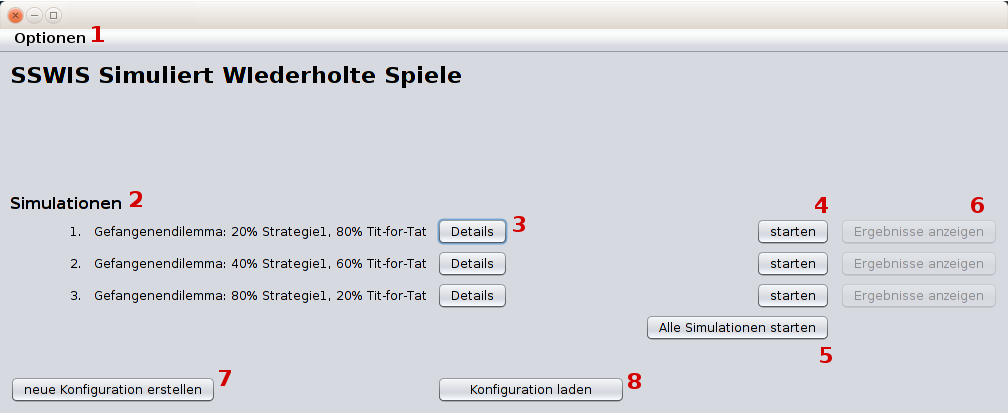
\includegraphics[width=1.1\textwidth]{GUI_Entwurf/StartfensterBeispiel.png}
  \caption{Hauptfenster}
  \label{fig:Bild1}
\end{figure}

\begin{description}


\item[1. Optionen] Menü enthält Zwei Untermenüs, Ergebnisse und Konfigurationen über die gespeicherte Ergebnisse und Startkonfigurationen angezeigt werden können

\item[2. Simulationen] Liste der geladenen Simulationen. Die wichtigsten Startkonfigurationen wie das Stufenspiel und die gewählten Strategien werden angezeigt.

\item[3. Details] Über diesen Knopf kann in einem Pop-Up-Fenster alle Parameter der Startkonfiguration eingesehen werden.

\item[4. starten] Die jeweilige Simulation kann über diesen Knopf ausgeführt werden. Wird die Simulation bereits ausgeführt oder ist sie in der Warteschlange, so ist der Knopf deaktiviert.

\item[5. Alle Simulationen starten] Durch diesen Knopf werden alle Simulationen, die nicht gerade ausgeführt oder bereits in der Warteschlange sind, nach einander ausgeführt. 

\item[6. Ergebnisse anzeigen] Bei Betätigung werden die Ergebnisse der jeweiligen Simulation der letzen Ausführung angezeigt. Wurde die Simulation noch nicht ausgeführt, ist der Knopf deaktiviert.

\item[7. neue Konfiguration erstellen] Führt zum Konfigurations-Assistenten, um alle Parameter für eine neue Startkonfiguration zu bestimmen.

\item[8. Konfiguration laden] Öffnet ein Dialogfenster, in dem man eine zuvor gespeicherte Konfiguration auswählen kann.

\end{description}


\subsection{Konfigurationen erstellen}

\begin{figure}[hp] 
  \centering
     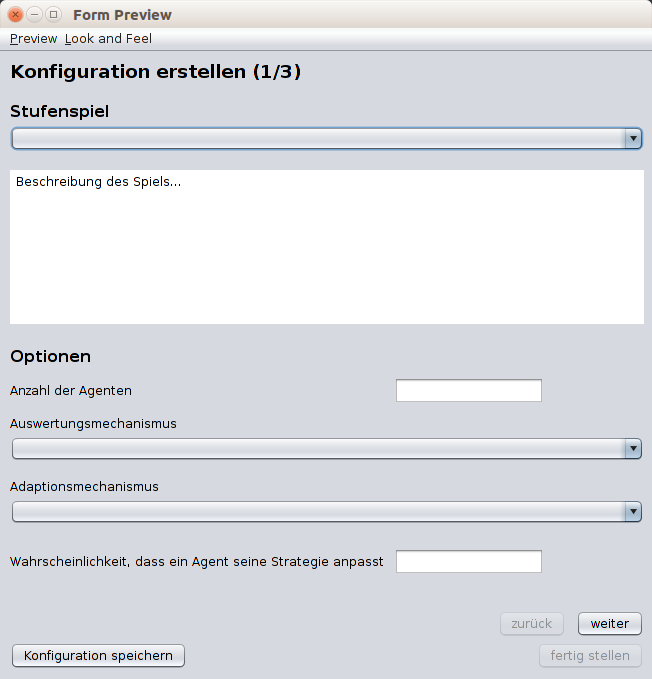
\includegraphics[width=1.0\textwidth]{GUI_Entwurf/WizardFenster1.png}
  \caption{Konfigurations-Assistent-Seite1}
  \label{fig:Bild2}
\end{figure}

\begin{description}

\item[1. Stufenspiel] Es kann ein Stufenspiel gewählt werden

\item[2. Beschreibung des Spiels] Wenn ein Stufenspiel gewählt ist, steht hier eine kurze Beschreibung unteranderem mit den unterschiedlichen Auszahlungen

\item[3. Anzahl der Agenten] Es werden nur gerade Zahlen akzeptiert

\item[4. Auswertungsmechanismus] Es kann zwischen den Auswertungsmechanismen gewählt werden.

\item[5. Adaptionsmechanismus] Es kann zwischen den Adaptionsmechanismen gewählt werden.

\item[6. Wahrscheinlichkeit] Hier kann eine Wahrscheinlichkeit größer als null und kleiner gleich 100 in Prozent angegeben werden, dass Agenten nach einem Zyklus ihre Startegie gegebenen falls anpassen.

\item[7. Konfiguration speichern] Es öffnet sich ein Dialogfenster, um einen Namen für die erstellt Konfiguration zu bestimmen.

\item[8. zurück] Ist auf dieser Seite deaktiviert.

\item[9. weiter] Führt zur nächsten Seite, wenn alle Parameter korrekt eingegeben wurden. Bei falschen oder fehlenden Eingaben gibt es eine Fehlermeldung.

\item[10. fertig stellen] Ist aktiviert wenn alle nötigen Eingaben auf dieser und den anderen zwei Seiten getätigt wurden. Wenn alle Eingaben korrekt sind, wird das Fenster geschlossen und die Simulationen werden auf die Startseite geladen. Bei falschen oder fehlenden Eingaben gibt es eine Fehlermeldung.

\end{description}

\pagebreak

\begin{figure}[hp] 
  \centering
     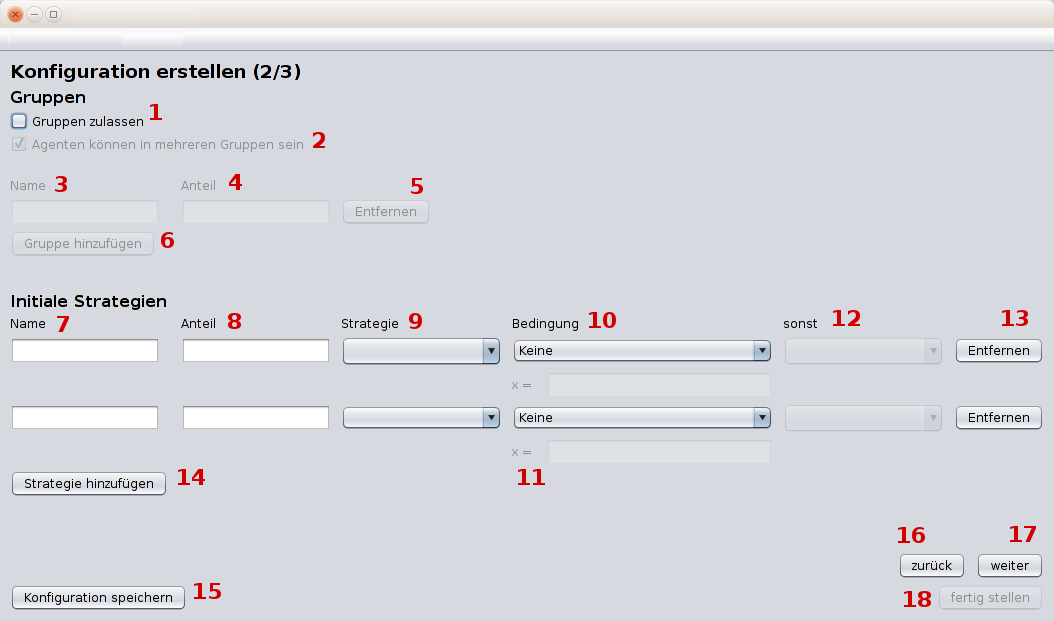
\includegraphics[width=1.1\textwidth]{GUI_Entwurf/WizardFenster2.png}
  \caption{Konfigurations-Assistent-Seite2}
  \label{fig:Bild3}
\end{figure}

\begin{description}

\item[1. Gruppen zulassen] Aktiviert die Felder 2 bis 6 und aktiviert Bedingung die sich auf Gruppen beziehen.

\item[2. Agenten können in mehreren Gruppen sein] Lässt Überlappungen von Gruppen zu.

\item[3. Name] Name der Gruppe.

\item[4. Anteil] Anteil der Agenten in dieser Gruppe zu Beginn des Spiels in Prozent. Es werden Eingaben größer als null und kleiner gleich 100 akzeptiert.

\item[5. Entfernen] Es kann zwischen den Adaptionsmechanismen gewählt werden.

\item[6. Gruppe hinzufügen] Fügt eine neue Zeile mit den Feldern 3 bis 5 an.

\item[7. Name] Name der erstellten Strategie.

\item[8. Anteil] Anteil der Agenten in dieser Gruppe zu Beginn des Spiels in Prozent. Es werden Eingaben größer als null und kleiner gleich 100 akzeptiert. Alle Anteil-Felder müssen zusammen 100 ergeben.

\item[9. Strategie] Wähle zwischen vier 'Basis-Strategien': Tit-for-Tat, Grim, keine Kooperation, immer Kooperation

\item[10. Bedingung] Wähle die Bedingung mit der die Strategie eintritt. 

\item[11. x] Falls die Bedingung 'mit Wahrscheinlichkeit x' gewählt ist kann hier die Wahrscheinlichkeit in Prozent eingegeben werden. Die Eingabe muss dann größer als null und kleiner gleich 100 sein. Falls die Bedingung 'mit Gruppe x' gewählt ist kann hier der Name der Gruppe eingegeben werden. Sonst ist das Feld deaktiviert.

\item[12. sonst] Hier kann die alternative 'Basis-Strategien' gewählt werden, die eintritt, wenn die erste Strategie nicht eintritt.

\item[13. entfernen] Alle Felder in dieser Zeile werden gelöscht.

\item[14. Strategie hinzufügen] Fügt eine neue Zeile an, mit den Feldern 7 bis 13.

\item[15. Konfiguration speichern] Es öffnet sich ein Dialogfenster, um einen Namen für die erstellt Konfiguration zu bestimmen.

\item[16. zurück] Führt zu der ersten Seite.

\item[17. weiter] Führt zur nächsten Seite, wenn alle Parameter korrekt eingegeben wurden. Bei falschen oder fehlenden Eingaben gibt es eine Fehlermeldung.

\item[18. fertig stellen] Ist aktiviert wenn alle nötigen Eingaben auf dieser und den anderen zwei Seiten getätigt wurden. Wenn alle Eingaben korrekt sind, wird das Fenster geschlossen und die Simulationen werden auf die Startseite geladen. Bei falschen oder fehlenden Eingaben gibt es eine Fehlermeldung.

\end{description}

\pagebreak

\begin{figure}[hp] 
  \centering
     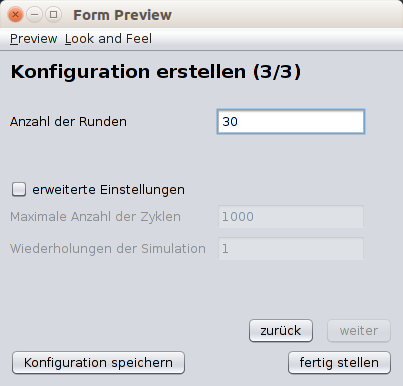
\includegraphics[width=0.7\textwidth]{GUI_Entwurf/WizardFenster3.png}
  \caption{Konfigurations-Assistent-Seite3}
  \label{fig:Bild4}
\end{figure}

\begin{description}

\item[1. Anzahl der Runden] Die Anzahl der Runden in einer Simulation. Es werden ganzzahlige Eingaben akzeptiert.

\item[2. erweiterte Eintellungen] Nur wenn der Haken gesetzt ist, sind die unteren zwei Felder 3 und  aktiviert.

\item[3. Maximale Anzahl der Zyklen] Maximale Anzahl der Zyklen, nachdenen die Simulation abgebrochen wird, auch wenn kein Gleichgewichtszustand erreicht wurde. Es werden ganzzahlige Eingaben akzeptiert.

\item[4. Wiederholungen der Simulation] Anzahl der Wiederholungen der ganzen Simulation. Es werden ganzzahlige Eingaben akzeptiert.

\item[5. Konfiguration speichern] Es öffnet sich ein Dialogfenster, um einen Namen für die erstellt Konfiguration zu bestimmen.

\item[6. zurück] Führt zur zweiten Seite.

\item[7. weiter] Ist auf dieser Seite deaktiviert.

\item[8. fertig stellen] Ist aktiviert wenn alle nötigen Eingaben auf dieser und den anderen zwei Seiten getätigt wurden. Wenn alle Eingaben korrekt sind, wird das Fenster geschlossen und die Simulationen werden auf die Startseite geladen. Bei falschen oder fehlenden Eingaben gibt es eine Fehlermeldung.

\end{description}


\subsection{Konfigurationen speichern und laden}

Die Dialogfenster zum speichern und laden von Ergebnissen werden sehr ähnlich aussehen.

\begin{figure}[hp] 
  \centering
     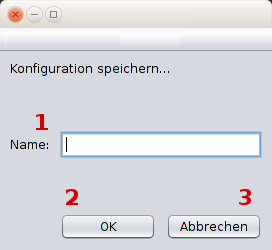
\includegraphics[width=0.5\textwidth]{GUI_Entwurf/KonfigSpeichern.png}
  \caption{Dialog: Konfiguration speichern}
  \label{fig:Bild5}
\end{figure}

\begin{description}

\item[1. Name] Name für die zu speichernde Konfiguration
\item[2. OK] Wurde ein Name eingegeben, so wird das Fenster geschlossen und alle durch den Assistenten eingegeben Parameter der Startkonfiguration unter diesem Namen gespeichert.
\item[3. Abbrechen] Der Vorgang wird abgebrochen und das Fenster schließt sich.

\end{description}

\pagebreak

\begin{figure}[hp] 
  \centering
     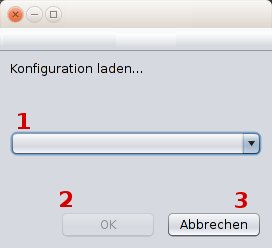
\includegraphics[width=0.5\textwidth]{GUI_Entwurf/KonfigLaden.png}
  \caption{Dialog: Konfiguration laden}
  \label{fig:Bild6}
\end{figure}

\begin{description}

\item[1. Konfiguration] Es kann zwischen den bereits gespeicherten Konfigurationen gewählt werden.
\item[2. OK] Wurde eine Konfiguration gewählt, so wird das Fenster geschlossen und der Assistent wird geöffnet. Alle gespeicherten Parameter der gewählten Konfiguration sind im Assistenten bereits eingegeben.
\item[3. Abbrechen] Der Vorgang wird abgebrochen und das Fenster schließt sich.

\end{description}

\pagebreak

\subsection{Ergebnisse anzeigen}

\begin{figure}[hp] 
  \centering
     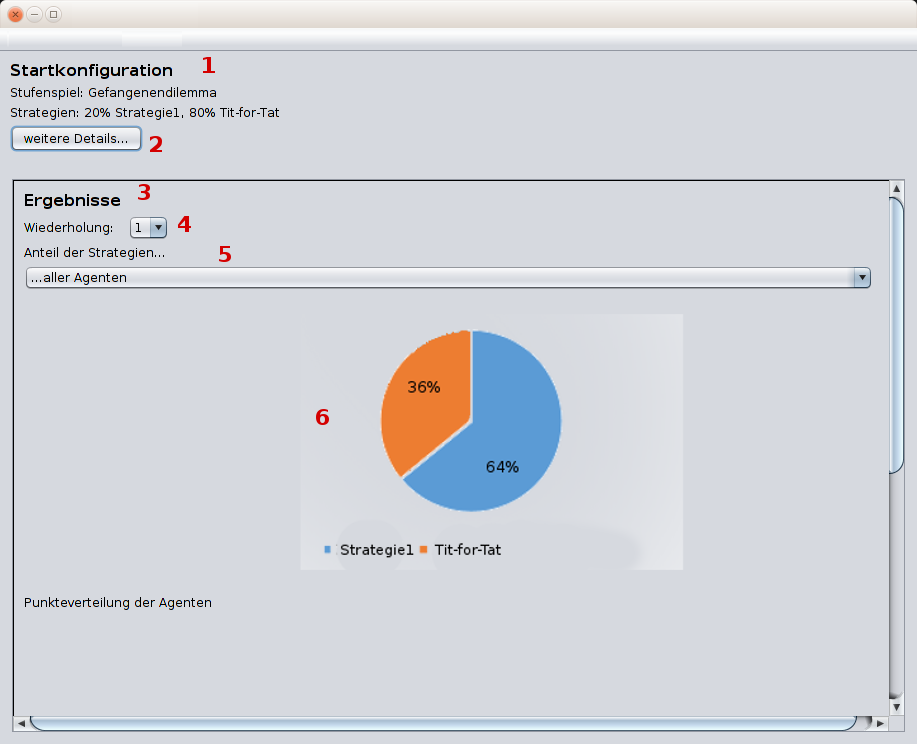
\includegraphics[width=1.1\textwidth]{GUI_Entwurf/Ergebnisfenster1.png}
  \caption{Ergebnisfenster1}
  \label{fig:Bild7}
\end{figure}

\begin{description}

\item[1. Startkonfiguartion] Die wichtigsten Parameter der Startkonfiguration werden angezeigt.

\item[2. Details] In einem Pop-Up-Fenster werden alle Parameter der Startkonfiguration angezeigt.

\item[3. Ergebnisse] Das Feld zum anzeigen der Ergebnisse lässt sich scrollen.

\item[4. Wiederholung] Es kann zwischen den einzelnen Wiederholungen der Simulation gewählt werden. D

\item[5. Anteil der Strategien] Anteil der Strategien aller Agenten am Ende der Simulation. 

\item[6. zurück] Zeigt den Anteil der Strategien aller Agenten am Ende der Simulation in einem Kuchendiagramm. 

\end{description}

\pagebreak

\begin{figure}[hp] 
  \centering
     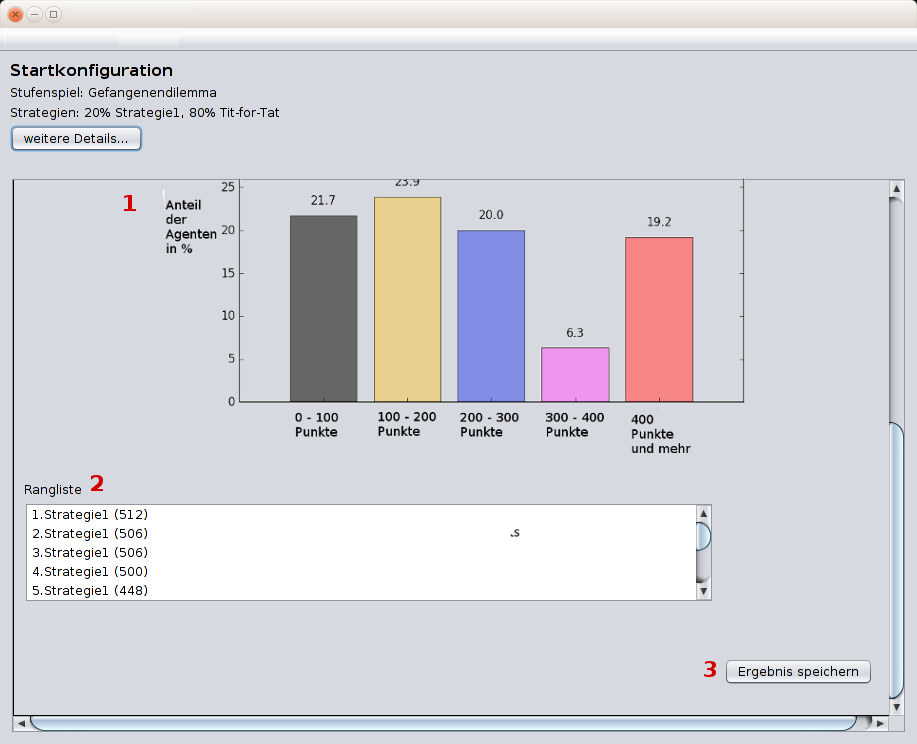
\includegraphics[width=1.1\textwidth]{GUI_Entwurf/Ergebnisfenster2.png}
  \caption{Ergebnisfenster2}
  \label{fig:Bild8}
\end{figure}

\begin{description}

\item[1. Punkteverteilung der Agenten] Zeigt die Verteilung der Summe aller Auszahlungen der Agenten am Ende der Simulation in einem Balkendiagramm an.

\item[2. Rangliste] Zeigt eine Rangliste aller Agenten am Ende der Simulation mit ihrem Rang ihre letzten Strategie und die Summe aller ihrer Auszahlungen.

\item[3. Ergebnisse speichern] Öffnet ein Dialogfenster in den ein Name für die Ergebnisse gewählt werden kann.


\end{description}



\section{Qualitätsbestimmungen}

\section{Globale Testfälle}

\subsection{Testfälle}



\textbf{/T001/} Konfiguration erstellen
\begin{enumerate}
\item \testfall{Das Startfenster ist geöffnet und es wird gerade keine Simulation durchgeführt.}
{Der Benutzer drückt auf den Button 'Konfiguration erstellen'.}
{Es öffnet sich die erste Seite des Konfigurations-Assistenten.}

\item \testfall{Die erste oder zweite Seite des Konfigurations-Assistenten ist geöffnet.}
{Der Benutzer tätigt alle Eingaben auf dieser Seite und mindestens eine der Eingaben ist nicht korrekt. Er bestätigt mit klicken auf 'weiter'.}
{Es kommt eine Fehlermeldung zu einer fehlerhaften Eingabe.}

\item \testfall{Die erste oder zweite Seite des Konfigurations-Assistenten ist geöffnet.}
{Der Benutzer tätigt alle Eingaben auf dieser Seite korrekt und bestätigt diese mit klicken auf 'weiter'.}
{Es wird die nächste Seite des Konfigurations-Assistenten geöffnet.}

\item \testfall{Eine Seite des Konfigurations-Assistenten ist geöffnet.}
{Der Benutzer tätigt alle Eingaben auf allen Seiten und mindestens eine der Eingaben ist nicht korrekt. Der Button 'fertig stellen' wird aktiviert und der Benutzer bestätigt mit klicken auf 'fertig stellen'.}
{Es kommt eine Fehlermeldung.}

\item \testfall{Eine Seite des Assistenten ist geöffnet.}
{Der Benutzer tätigt alle Eingaben auf allen Seiten korrekt und bestätigt diese mit klicken auf 'fertig stellen'.}
{Das Fenster schließt sich und die erstellten Konfigurationen werden auf die Startseite geladen.}


\end{enumerate}

\textbf{/T002/} Konfigurationen speichern und laden
\begin{enumerate}
\item \testfall{Das Startfenster ist geöffnet und es wird gerade keine Simulation durchgeführt}
		{Der Benutzer klickt auf den Button 'Konfiguration laden' und wählt eine in der Liste genannten Konfigurationen. Er bestätigt mit 'OK'}
		{Es öffnet sich der Konfigurations-Assistent. Alle unter dem gewählten Namen gespeicherten Parameter sind bereits eingegeben.}
		
\item \testfall{Das Startfenster ist geöffnet und es wird gerade keine Simulation durchgeführt}
		{Der Benutzer wählt in dem Menü 'Optionen' das Untermenü 'Konfigurationen' und wählt eine der aufgelisteten Konfigurationen.}
		{Es öffnet sich der Konfigurations-Assistent. Alle unter dem gewählten Namen gespeicherten Parameter sind bereits eingegeben.}

\item \testfall{Eine Seite des Konfigurations-Assistenten zum erstellen einer Konfiguration ist geöffnet.}
		{Der Benutzer klickt auf den Button 'Konfiguration speichern'. In dem sich geöffneten Pop-Up-Fenster gibt er einen Namen für die Konfiguration ein und bestätigt mit 'OK'}
		{Das Fenster sowie der Assistent schließen sich.}
\end{enumerate}

\textbf{/T003/} Simulationen starten
\begin{enumerate}
\item \testfall{Das Startfenster ist geöffnet und es wird mindestens eine Simulation in der Liste 'Simulationen' angezeigt, die aktuell nicht durchgeführt wird.}
		{Der Benutzer klickt auf den Button 'start' neben einer Simulation.}
		{Der Button 'start' wird deaktiviert. Nachdem die Simulation beendet ist, wird der Button 'start' und 'Ergebnisse anzeigen' aktiviert.}
		
\item \testfall{Das Startfenster ist geöffnet und es wird mindestens eine Simulation in der Liste 'Simulationen' angezeigt, die aktuell nicht durchgeführt wird.}
		{Der Benutzer klickt auf den Button 'Alle Simulationen starten'}
		{Alle 'start' Knöpfe und der Button 'Alle Simulationen starten' werden deaktiviert. Nachdem die Simulationen beendet wurden, werden alle 'start' Knöpfe, alle 'Ergebnisse anzeigen' und der Button 'Alle Simulationen starten' aktiviert.}
\end{enumerate}

\textbf{/T004/} Ergebnisse anzeigen
\begin{enumerate}
\item \testfall{Das Startfenster ist geöffnet und es wird mindestens eine Simulation in der Liste 'Simulationen' angezeigt, die bereits durchgeführt wurde.}
		{Der Benutzer klickt auf 'Ergebnisse anzeigen'.}
		{Es öffnet sich das Ergebnisfenster der Simulation.}
\end{enumerate}

\textbf{/T005/} Ergebnisse speichern und laden
\begin{enumerate}
\item \testfall{Das Ergebnisfenster einer Simulation ist geöffnet.}
		{Der Benutzer scrollt bei den Ergebnissen ganz nach unten und drückt auf Ergebnisse speichern. Im geöffneten Pop-Up-Fenster gibt er einen Namen ein und bestätigt auf 'OK'.}
		{Das Pop-Up-Fenster schließt sich.}

\item \testfall{Das Startfenster ist geöffnet.}
		{Der Benutzer wählt in dem Menü 'Optionen' das Untermenü 'Konfigurationen' und wählt eine der aufgelisteten Ergebnisse.}
		{Es öffnet sich das Ergebnisfenster des gespeicherten Ergebniszustands.}
\end{enumerate}




\section{Systemmodelle}

\subsection{Szenarien}

\subsubsection{Eigenes Spiel erstellen}
Der Benutzer möchte ein Spiel erstellen, das beide Spieler dafür belohnt, unterschiedliche Entscheidungen zu treffen.\\
Hierfür öffnet er das Spiele-Menü und klickt auf 'neues Spiel'. Er gibt dem Spiel einen Namen und setzt die Werte:
\begin{table}[H]
\centering
\setlength{\extrarowheight}{2pt}
\begin{tabular}{cc|c|c|}
  & \multicolumn{1}{c}{} & \multicolumn{2}{c}{Spieler $2$} \\
  & \multicolumn{1}{c}{} & \multicolumn{1}{c}{$K$} & \multicolumn{1}{c}{$D$} \\\cline{3-4}
  \multirow{2}*{Spieler $1$} & $K$ & $0,0$ & $3,3$ \\\cline{3-4} 
  & $D$ & $3,3$ & $0,0$ \\\cline{3-4}
\end{tabular}
\end{table}
Anschließend versieht er sein Spiel mit einer Beschreibung.\\
Er beendet den Vorgang durch Klicken von 'Änderungen speichern und schließen'.

\subsubsection{Kombinierte Strategie erstellen}
Der Benutzer möchte eine eigene kombinierte Strategie erstellen, bei der Agenten eine besondere Verhaltensweise gegenüber Agenten innerhalb ihrer Gruppe und gegenüber reicheren Agenten außerhalb ihrer Gruppe haben.\\
Hierfür öffnet er das Spiele-Menü und klickt auf 'neue kombinierte Strategie'. Er gibt der Strategie den Namen "`GruppenTitforTat"'. Unter 'Bedingungen' klickt er auf 'hinzufügen'. Er wählt die Bedingung 'Mit meiner Gruppe' und die Strategie 'Tit for Tat'.
Analog fügt er eine weitere Bedingung 'Mit reicheren Agenten' mit der Strategie 'Grim' hinzu. Für 'keine Bedingung' wählt er 'keine Kooperation'. Schließlich beschreibt er in einem Textfeld seine Strategie und klickt 'kombinierte Strategie speichern und schließen'.

\subsubsection{Rivalisierende Gruppen}
Der Benutzer möchte eine Population mit zwei rivalisierenden Gruppen simulieren.\\
Hierfür hat er bereits eine kombinierte Strategie erstellt, nach der Agenten mit Agenten aus ihrer eigenen Gruppe kooperieren, mit Agenten aus einer anderen Gruppe nicht kooperieren und sonst 'Tit for Tat' spielen.\\
Im Initialisierungsmenü erstellt er nun zwei Gruppen und gibt unter 'Anteil aller Agenten' den Wert 25 ein. Beiden Gruppen weist er seine Strategie zu, allen anderen 'Tit for Tat'.

\subsubsection{Ausreißer im Ergebnis vermeiden}
Der Benutzer hat sich für eine bestimmte Konfiguration entschieden, mit der er eine Simulation durchführen möchte. Um das Risiko von Ausreißern im Ergebnis zu verringern, wählt er beim Start der Simulation eine hohe Wiederholungsanzahl aus. Nach die Simulation abgeschlossen ist, wählt er in der Ergebnisansicht unter 'Wiederholung' den Punkt 'Durchschnitt' aus.

\newpage

\subsection{Anwendungsfälle}

\begin{figure}[htbp]
{\centering 
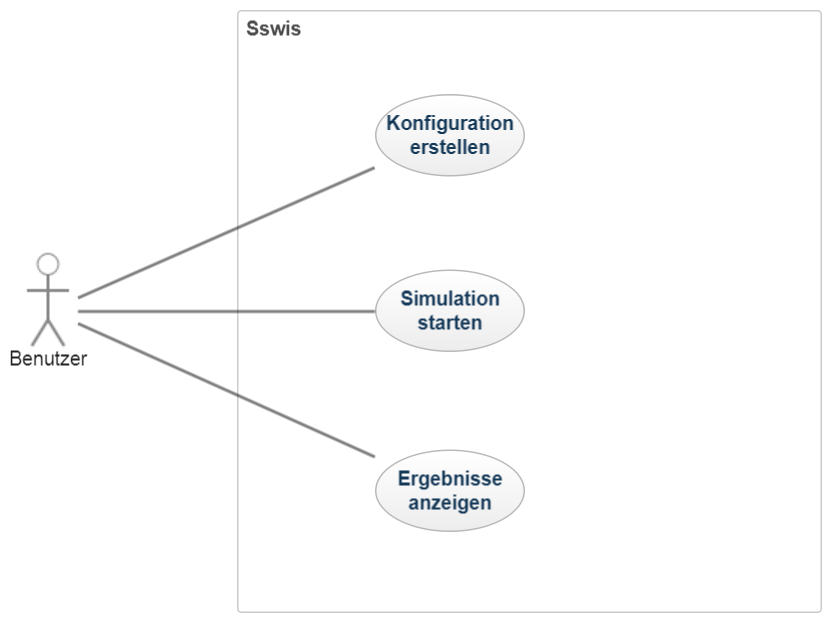
\includegraphics[width=0.9\textwidth]{Anwendungsfalldiagramme/usecase_sswis.png}
\caption{Das Programm in der Standardausführung} }
\bigskip
Sswis ist ein Simulator und gliedert sich als solcher in drei übergeordnete Anwendungen. Die Konfiguration der Rahmenbedingungen, das Starten der eigentlichen Simulation und das Abrufen der Ergebnisse. Die Interaktion mit dem Benutzer beschränkt sich im Wesentlichen auf die Konfiguration und die Anzeige der Ergebnisse Außerdem kann er die für die Konfiguration verfügbaren Spiele und Strategien verwalten\footnotemark. Die Simulation wird vom Benutzer initiiert und läuft anschließend ohne weiteres Einwirken von außen ab.

\end{figure}

\footnotetext{darin inbegriffen sind Möglichkeiten zur Benennung, Erstellung und Löschung für sowohl Spiele als auch Strategien}

\begin{figure}[htbp]
{\centering
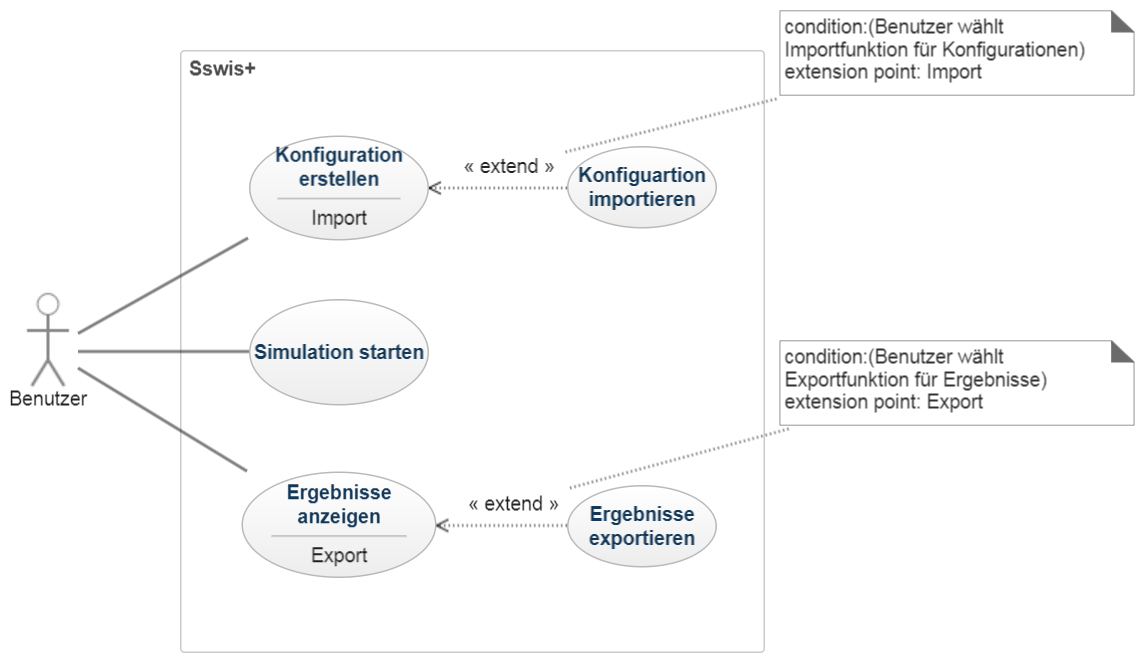
\includegraphics[width=1.0\textwidth]{Anwendungsfalldiagramme/usecase_sswis+.png}
\caption{Das Programm mit allen optionalen Funktionen} }
\bigskip

Zusätzlich zum Funktionsumfang von Sswis, erlaubt Sswis+ das Importieren von Konfigurationen und Initialisierungen und das Exportieren von Ergebnissen in Form jeweils einer Textdatei (z.B. CSV; Comma-separated values). Dateien zum Import einer Konfiguration bzw. Initialisierung wurden zu einem früheren Zeitpunkt durch den entsprechenden Assistenten erstellt.

\end{figure}

\section{Glossar}

\textbf{Spiel}
Ein spieltheoretisches Stufenspiel, welches sich als 2x2 Matrix darstellen lässt, wobei sich an jeder der 4 Einträge die Payoffs für beide Spieler befinden.

\textbf{Strategie}
Eine Strategie eines Agenten A bestimmt die Aktion von A im Verlauf eines Spiels mit einem Agenten B. Die Strategie kann von den vergangenen Aktionen des Agenten B, den Rängen von A und B, sowie deren Gruppenzugehörigkeit abhängen. Die Strategie eines Agenten kann sich während der Simulation ändern.

\textbf{Runde}
Eine Runde umfasst die Paarung aller Agenten und das einmalige Spielen des ausgewählten Stufenspiels.

\textbf{Zyklus}
Ein Zyklus umfasst $k$ Runden sowie das Auswerten und Anpassen der Strategien.

\textbf{Gruppe}
Eine Gruppe ist eine Menge von Agenten, die vom Benutzer festgelegt werden kann.

\textbf{Gleichgewicht}
Ein Gleichgewicht bezeichnet den Zustand, in dem die Agenten in den letzten 500 Zyklen ihre Strategie nicht mehr angepasst haben.

\textbf{reicher und ärmer}
Ein Agent A ist reicher bzw. ärmer als ein Agent B, wenn er mehr bzw. weniger Punkte hat.

\textbf{ungefähr gleich reich}
Zwei Agenten sind ungefähr gleich reich, wenn die Differenz ihrer Punkte $\pm 50$ Punkte beträgt.

\textbf{Konfiguration}
Eine Menge von Parametern, die eine Simulation oder eine Menge von Simulationen\footnote{vgl. /F0210/} beschreibt.


\end{document}